\documentclass[a4paper,12pt]{article}

%%% Работа с русским языком
\usepackage{cmap}					% поиск в PDF
\usepackage{mathtext} 				% русские буквы в формулах
\usepackage[T2A]{fontenc}			% кодировка
\usepackage[utf8]{inputenc}			% кодировка исходного текста
\usepackage[english,russian]{babel}	% локализация и переносы

%%% Дополнительная работа с математикой
\usepackage{amsmath,amsfonts,amssymb,amsthm,mathtools} % AMS
\usepackage{icomma} % "Умная" запятая: $0,2$ --- число, $0, 2$ --- перечисление

%% Номера формул
%\mathtoolsset{showonlyrefs=true} % Показывать номера только у тех формул, на которые есть \eqref{} в тексте.
%\usepackage{leqno} % Нумерация формул слева

%% Свои команды
\DeclareMathOperator{\sgn}{\mathop{sgn}}

%% Перенос знаков в формулах (по Львовскому)
\newcommand*{\hm}[1]{#1\nobreak\discretionary{}
{\hbox{$\mathsurround=0pt #1$}}{}}

%%% Работа с картинками
\usepackage{graphicx}  % Для вставки рисунков
\graphicspath{{materials}{images2/}}  % папки с картинками
\setlength\fboxsep{3pt} % Отступ рамки \fbox{} от рисунка
\setlength\fboxrule{1pt} % Толщина линий рамки \fbox{}
\usepackage{wrapfig} % Обтекание рисунков текстом

%%% Работа с таблицами
\usepackage{array,tabularx,tabulary,booktabs} % Дополнительная работа с таблицами
\usepackage{longtable}  % Длинные таблицы
\usepackage{multirow} % Слияние строк в таблице

%%% Теоремы
\theoremstyle{plain} % Это стиль по умолчанию, его можно не переопределять.
\newtheorem{theorem}{Теорема}[section]
\newtheorem{proposition}[theorem]{Утверждение}
 
\theoremstyle{definition} % "Определение"
\newtheorem{corollary}{Следствие}[theorem]
\newtheorem{problem}{Задача}[section]
 
\theoremstyle{remark} % "Примечание"
\newtheorem*{nonum}{Решение}

%%% Программирование
\usepackage{etoolbox} % логические операторы

%%% Страница
%\usepackage{extsizes} % Возможность сделать 14-й шрифт
\usepackage{geometry} % Простой способ задавать поля
	\geometry{top=25mm}
	\geometry{bottom=30mm}
	\geometry{left=25mm}
	\geometry{right=25mm}
 %

%%% Способ сделать тоже самое(но красивее:)
%\usepackage[margin=0.8in]{geometry}

 
\usepackage{fancyhdr} % Колонтитулы
 	\pagestyle{fancy}
 	\renewcommand{\headrulewidth}{0mm}  % Толщина линейки, отчеркивающей верхний колонтитул
 	\lfoot{}
 	\rfoot{}
 	\rhead{}
 	\chead{}
 	\lhead{ }
 	% \cfoot{Нижний в центре} % По умолчанию здесь номер страницы

\usepackage{setspace} % Интерлиньяж
%\onehalfspacing % Интерлиньяж 1.5
%\doublespacing % Интерлиньяж 2
%\singlespacing % Интерлиньяж 1

\usepackage{lastpage} % Узнать, сколько всего страниц в документе.

\usepackage{soulutf8} % Модификаторы начертания

\usepackage{hyperref}
\usepackage[usenames,dvipsnames,svgnames,table,rgb]{xcolor}
\hypersetup{				% Гиперссылки
    unicode=true,           % русские буквы в раздела PDF
    pdftitle={Заголовок},   % Заголовок
    pdfauthor={Автор},      % Автор
    pdfsubject={Тема},      % Тема
    pdfcreator={Создатель}, % Создатель
    pdfproducer={Производитель}, % Производитель
    pdfkeywords={keyword1} {key2} {key3}, % Ключевые слова
    colorlinks=true,       	% false: ссылки в рамках; true: цветные ссылки
    linkcolor=red,          % внутренние ссылки
    citecolor=green,        % на библиографию
    filecolor=magenta,      % на файлы
    urlcolor=blue           % на URL
}

%\renewcommand{\familydefault}{\sfdefault} % Начертание шрифта

\usepackage{multicol} % Несколько колонок

% Мои "дополнительные" пакеты
\usepackage{textcase} 
\usepackage{pdfpages}
\usepackage{amsmath}
\usepackage{titlesec}
\usepackage{floatrow}

\usepackage{subfig}

\author{Подкидышев Алексей}
\title{Студент МФТИ ФИВТ - 3ий курс}
\date{\today}

%% Делаем красивый header:
\fancyhead[RO]{\footnotesize{\scshape\nouppercase{~\leftmark}}}
%% Делаем красивый header END

%Делаем большой отступ между section и subsection
\titlespacing*{\section} {0pt}{3.5ex plus 1ex minus .2ex}{2.7ex plus .2ex}
\titlespacing*{\subsection} {0pt}{2.7ex plus 1ex minus .2ex}{1ex plus .2ex}


\begin{document} % конец преамбулы, начало документа

\begin{center}
	\textit{\MakeTextUppercase{федеральное государственное автономное учреждение}}
		
	\vspace{0.5ex}
	
	\textbf{ \\ \MakeTextUppercase{<<Московский Физико-технический институт>>}}
\end{center}
\vspace{13ex}
\begin{flushright}
	\noindent
	{Подкидышев Алексей}
	\\
	\textit{Студенты факультета инноваций\\ и высоких технологий\\(группа 792)}
\end{flushright}
\begin{center}
	\vspace{23ex}
	\line(1,0){430}\\[4ex]
	{\LARGE\textbf{Лабораторная работа 7.4}}
	\vspace{2ex}\\
	\textbf{\large{<<Эллектронный >>}}\\[3ex]
	\line(1,0){430}\\[5ex]
	\vfill
	Долгопрудный 
	
	{\today}
\end{center}

\newpage
\newpage
\renewcommand{\headrulewidth}{1pt}

\section{Описание работы}


\begin{multicols}{2}
[
\subsection{Экспериментальная установка}
]
Установка (см. рис.5) состоит из двух детекторов частиц осцинтилляционных счетчиков из полистирола со сцинтиллирующими добавками, набора свинцовых и железных фильтров и
электронных схем, служащих для регистрации и дискриминации
сигналов от детекторов. Детекторы с размером чувствительной
части 40х 10х2,5 см размешены на базе около 40см. Регистрация световых вспышек от сцинтилляторов производится с помощью ФЭУ-85, напряжение питания (1000 В) на каждый ФЭУ
подается от стабилизированного высоковольтного выпрямителя.
Сигналы с ФЭУ поступают на усилителиформирователи, а затем
на схему двойных совпадений. Схема совпадений формирует на выходе сигналы
только в том случае, если в обоих детекторах
появились сигналы, совпадающие во времени в интервале, равном разрешающему времени схемы. В данной установке разрешающее время $\tau = 10 s$. Число зарегистрированных импульсов
регистрируется пересчетным прибором
\end{multicols}

\begin{figure}[h]
        \includegraphics[width=0.7 \textwidth]{Materials/ust.png}
    \caption{Схема установки}
\end{figure}

%%%%%%%%%%%%%%%%
\newpage
\subsection{Выдержка формул и графиков}

\begin{minipage}{0.45\textwidth}
\end{minipage}
\hfill
\begin{minipage}{0.45\textwidth}
\end{minipage}

\begin{figure}[htp] 
    \centering
    \subfloat[][Распределение мюонов по импульсам на уровне моря]{
        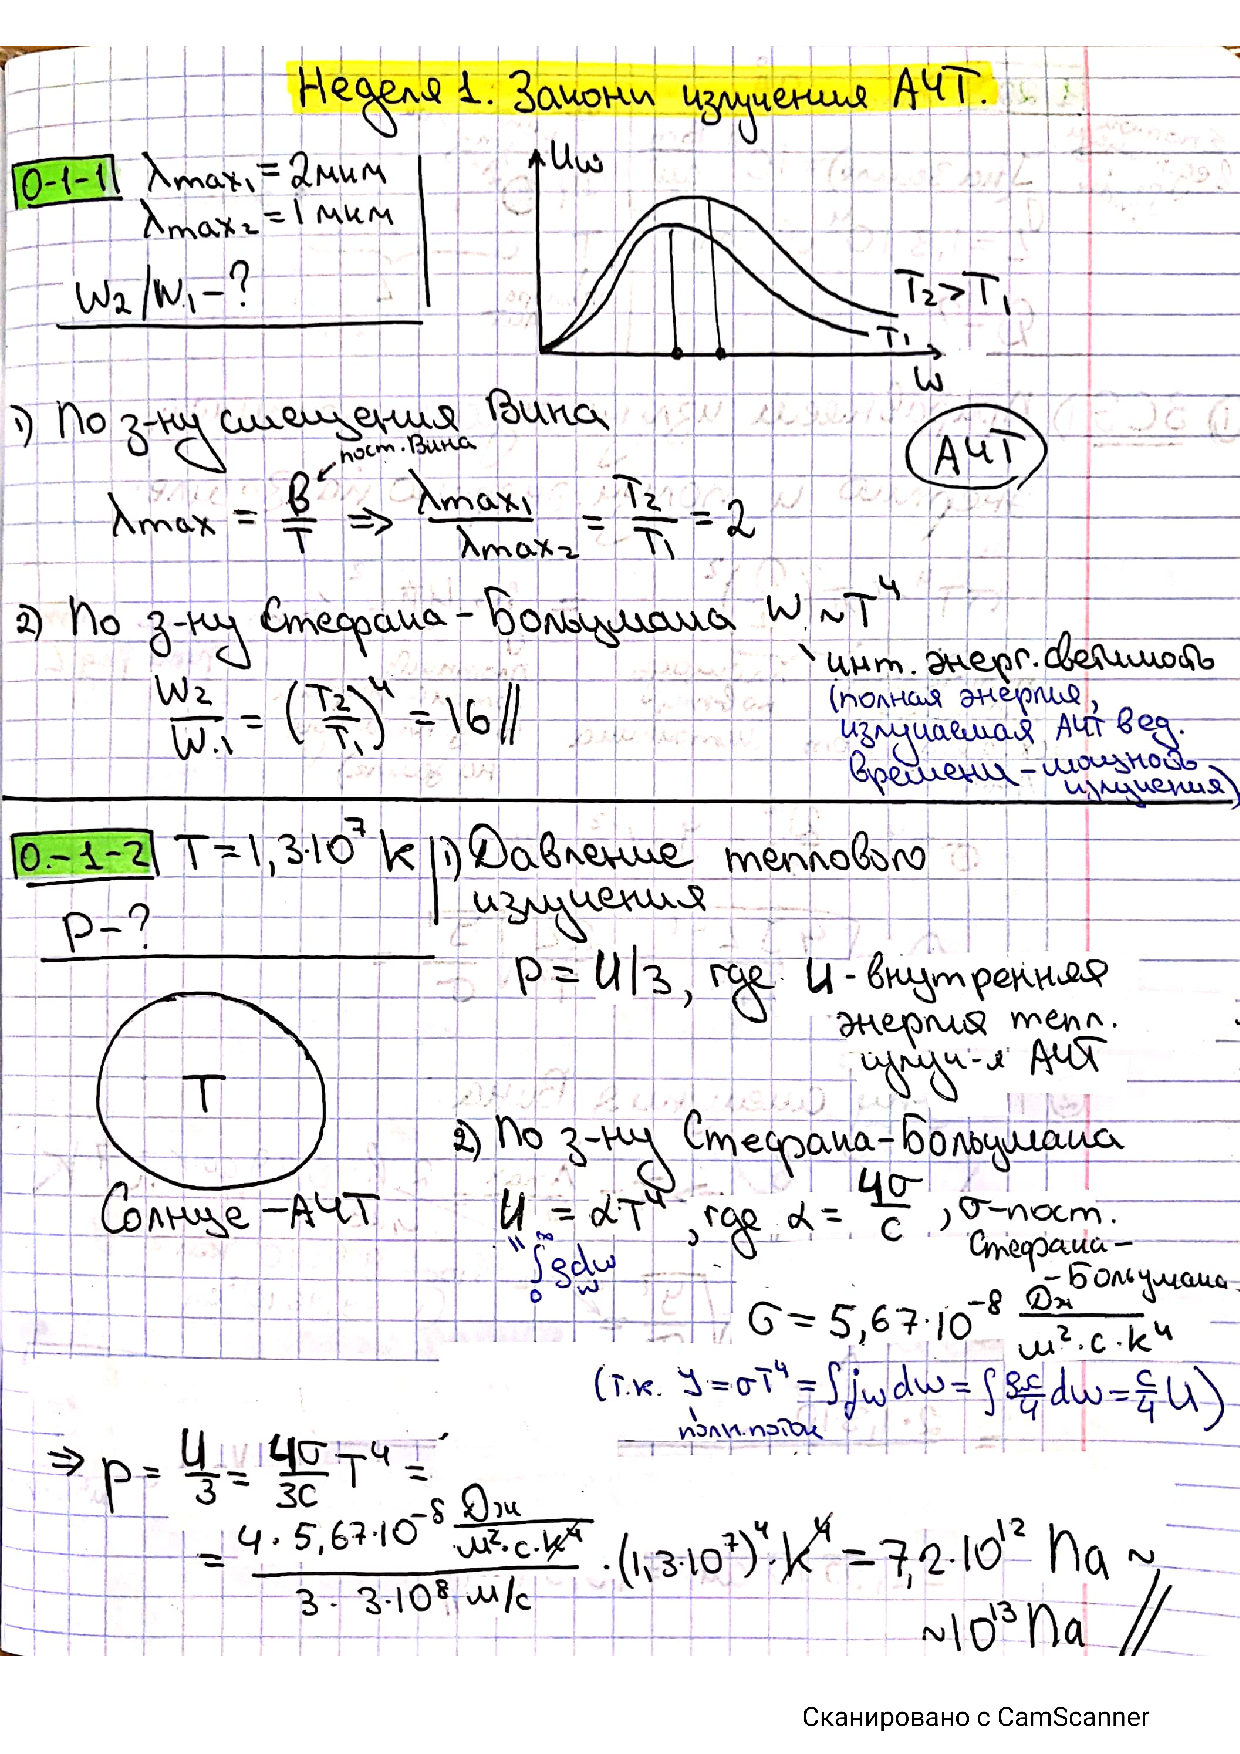
\includegraphics[width=0.4\textwidth]{Materials/1.png}
        }%
    \hfill%
    \subfloat[][Зависимость ионизационных потерь в различных веществеах от величины $p/mc = \beta / \sqrt{1 - \beta^2}$]{%
        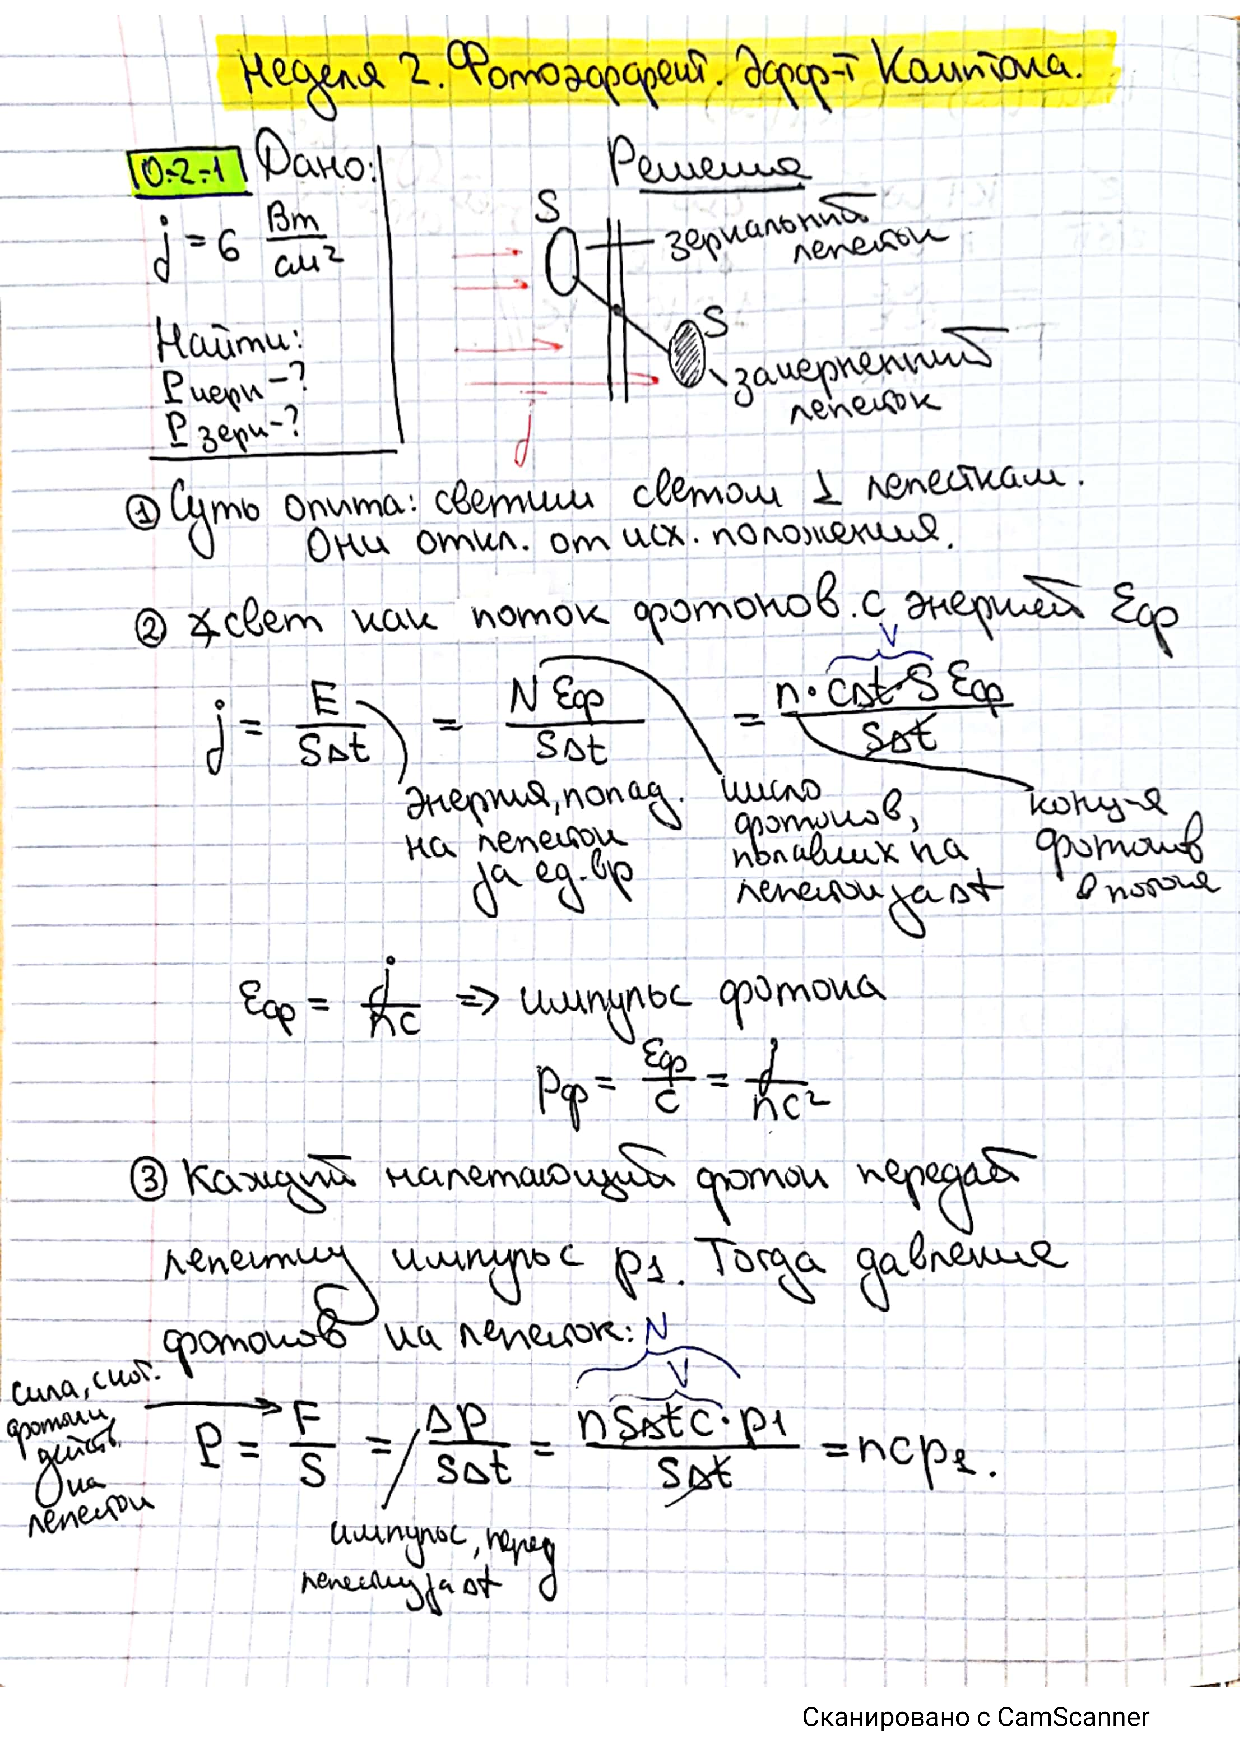
\includegraphics[width=0.4\textwidth]{Materials/2.png}
        }

    \subfloat[][Вклад различных процессов в сечение поглощения гамма квантов в свинце]{
        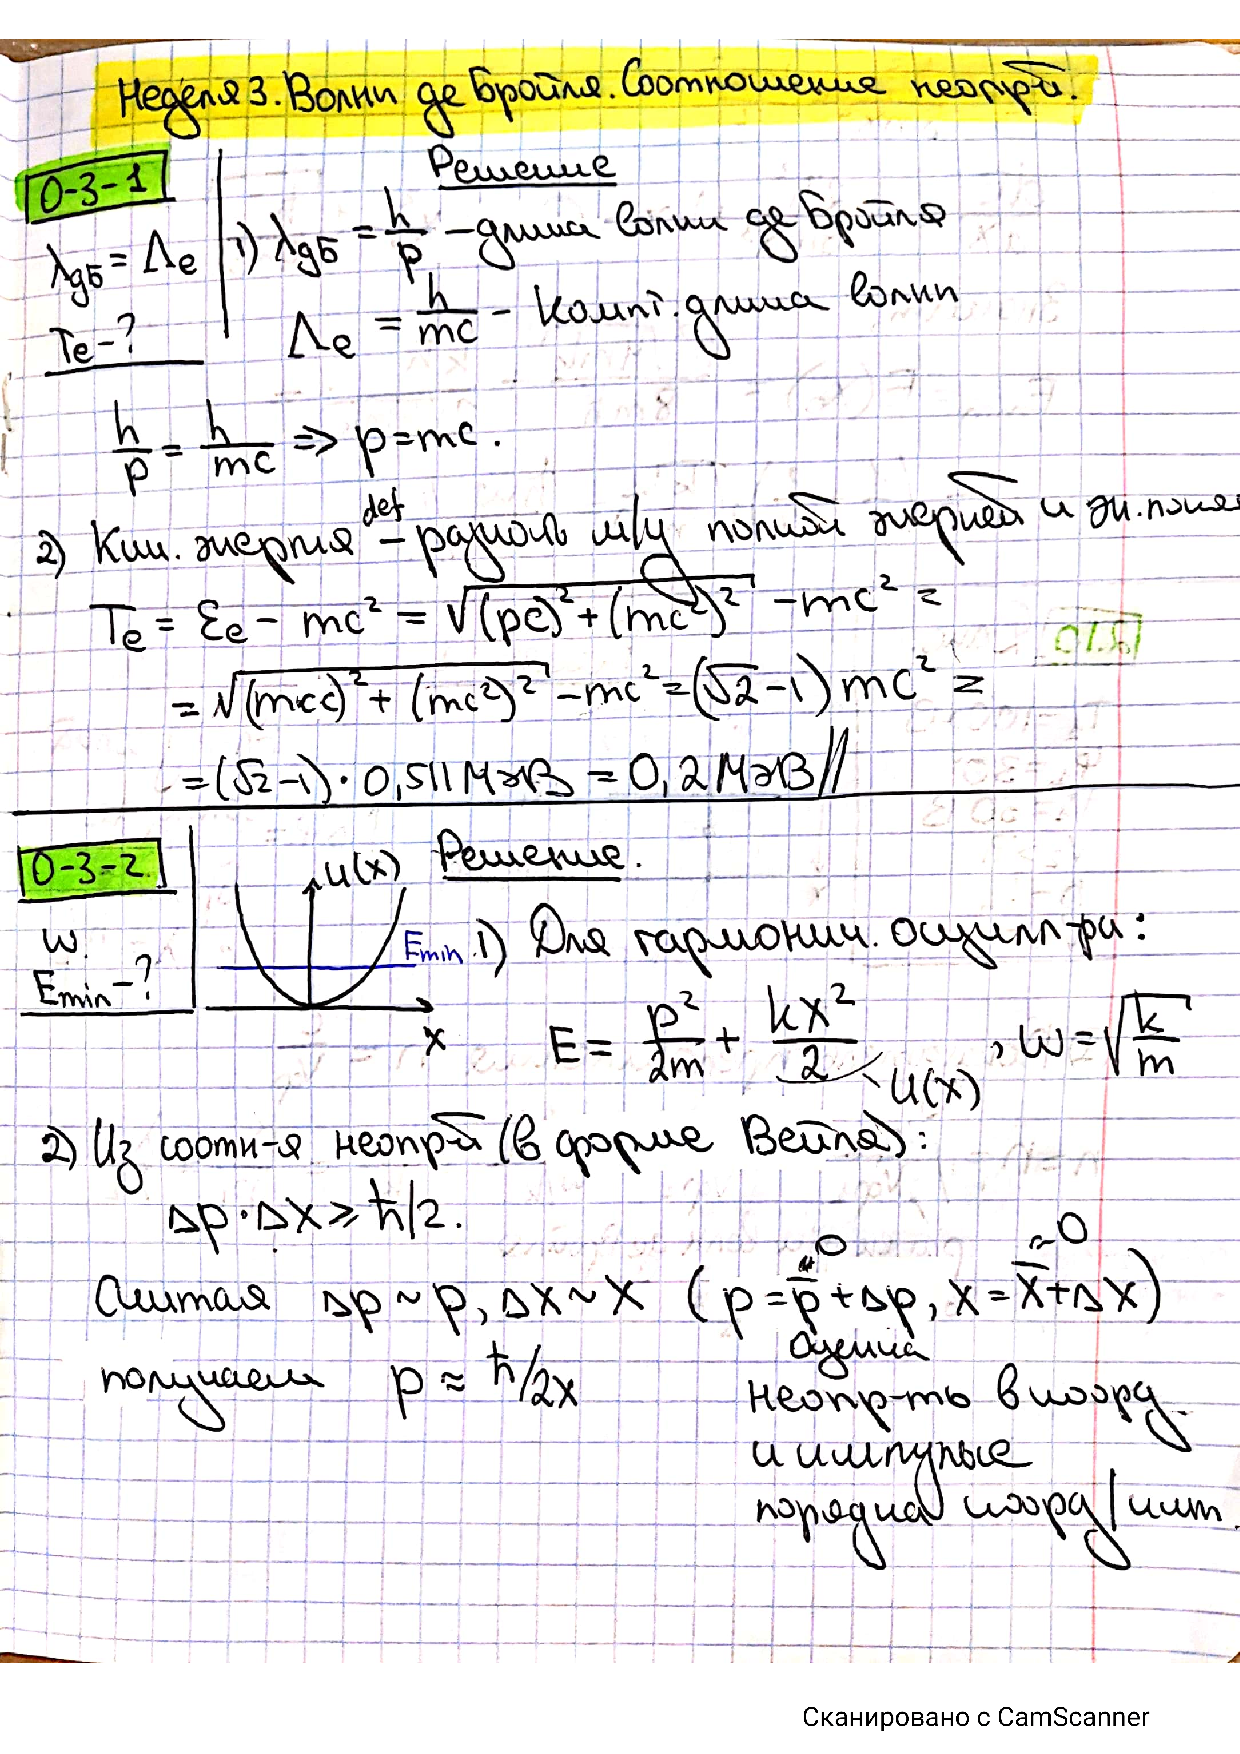
\includegraphics[width=0.4 \textwidth]{Materials/3.png}
        }
        
     \caption{Теоретические графики}   
\end{figure}



\newpage

Формула для полного сечения образования пары фотоном с энергией $h \nu$ имеет вид:
\[\sigma_\text{пар} = \dfrac{28}{9} Z^2 \alpha \big(\dfrac{e^2}{mc^2} \big)^2 \big[\ln{\dfrac{2 h \nu}{mc^2}} - \dfrac{109}{42} - (\alpha Z)^2 \big],  \] где Z - заряд ядра, $\alpha = e^2 / h c$ - постоянная тонкой структуры, которой всегда характеризуеются электрмагнитные процессы, а $r_0 = e^2/mc^2$ - классический радиус электрона.

\begin{figure}[H]
    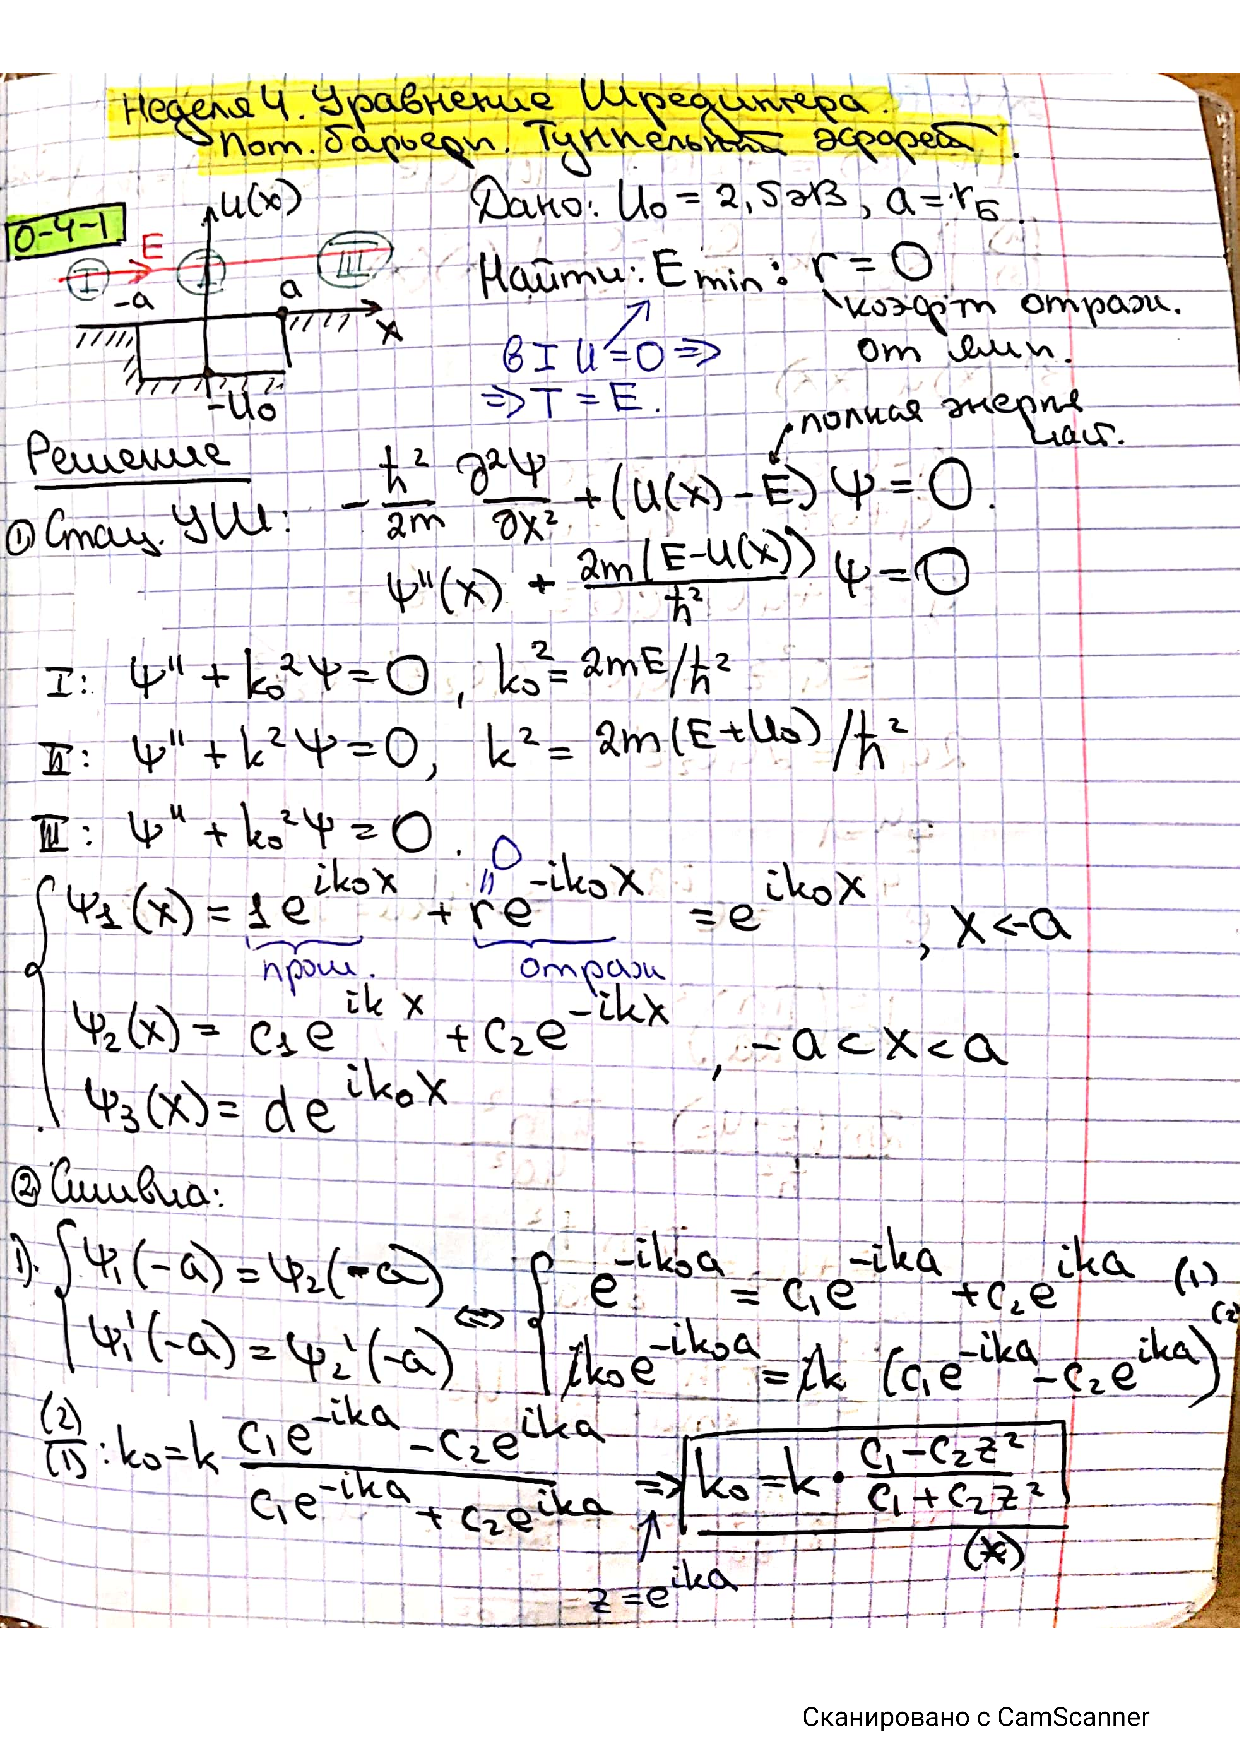
\includegraphics[width=0.4 \textwidth]{Materials/4.png}
    \caption{Зависимость эффективного сечения рождения пар на свинце и алюминии от энергии E гамма-кванта ($\Phi = Z^2 \alpha(e^2/mc^2)^2$) }
        
\end{figure}

\section{Ход Работы}
\begin{enumerate}
    \item Измерим фон каждого детектора в отдельности. Для детектора 1: $13.5,$ для детектора 2: $7.3.$ Так как для нашей установки разрешающее время $\tau = 10^{-7} c,$ то 
    \[I_{\text{сл}} = 2 \tau I_1 \cdot I_2 = 2 \cdot 10^{-7} \cdot 7.3 \cdot 13.5 = 2\cdot 10^{-5}.\]
    \item Снимем зависимость интесивности космического излучения от толщины проходимого ими вещества.


\begin{table}[H]
\caption{Зависимость интенсивности космического излучения от толщины проходимого им вещества}
\begin{tabular}{|l|l|}
\hline
\rowcolor[HTML]{FCFF2F} 
D, мм & I    \\ \hline
0     & 2.17 \\ \hline
20    & 1.83 \\ \hline
40    & 1.77 \\ \hline
60    & 1.70 \\ \hline
80    & 1.57 \\ \hline
100   & 1.55 \\ \hline
120   & 1.53 \\ \hline
\end{tabular}
\end{table}
    \newpage
    \item Построим график 
    
    \begin{figure}[H]
        \includegraphics[width= \textwidth]{Materials/graph/chart.png}
        \caption{Зависимость интенсивности космического излучения от толщины проходимого им вещества. Кривая проведена стандартными средствами MS EXCEL }
        
    \end{figure}
    
    \item Найдем отношение мягкой и жесткой компонент излучения:
    \[\frac{I_{\text{м}}}{I_\text{ж}} = \frac{I_\text{max} - I_\text{min}}{I_\text{min}} = \frac{2.17 - 1.53}{1.53} = 0.42.\]
\end{enumerate}

\section{Вывод}
Исследовали поглощение вторичного космического излучния, получили экспериментально график зависимости интенсивности излучения от толщины проходимого им вещества, также нашли отношение $\frac{I_{\text{м}}}{I_\text{ж}} = 0.42.$

\end{document}